\documentclass{article}

\usepackage{epsfig}  
\usepackage{amsmath} 
\usepackage{amssymb} 
\usepackage{amsthm}  
\usepackage{listings} 
\usepackage{color}
%\usepackage{enumerate}
\usepackage{enumitem}
\usepackage{multirow}
\usepackage{lastpage}
\usepackage{geometry}
\usepackage{fancyhdr}
\usepackage[all]{xy}
\usepackage{wrapfig}
\usepackage{listings}
\usepackage{url}
\usepackage{tikz}
\usepackage{graphicx}
\usepackage{caption}
\usepackage{subcaption}
\usepackage[justification=centering]{caption}
\usetikzlibrary{arrows}
\lstset{language=C, tabsize=4, basicstyle=\ttfamily}

\definecolor{light}{gray}{.75} 
\newtheorem{theorem}{Theorem}



\pagestyle{fancy}
\lhead{CSCE 990 - FALL 2014} 
\chead{\bfseries PROJECT PROPOSAL}
\rhead{Gerrard, Ore}
\lfoot{Gerrard, Ore}
\cfoot{\thepage\ of \pageref{LastPage}}
\rfoot{3 November 2014}
\renewcommand{\headrulewidth}{0.4pt}
\renewcommand{\footrulewidth}{0.4pt}

\hoffset 0pt
\voffset 0pt
\textwidth 15cm
\textheight 8.5in
\oddsidemargin 9pt
\marginparwidth 25pt
\setlength{\parindent}{0pt}
\setlength{\parskip}{.25cm}

%- - - - - - - - - - - - - - - - BEGIN DOCUMENT - - - - - - - - - - - - - - - - - - - 
\begin{document}


\section{Target Problem Description}
\cite{schneider2010synoptic}

\section{Sketch of technique}

%\begin{figure}[b]
    %\centering
    %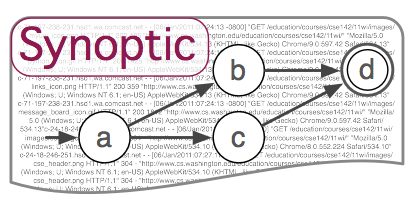
\includegraphics[width=0.4\textwidth]{./figures/TBD.jpg}
    %\caption{Awesome Image}
    %\label{fig:awesome_image}
%\end{figure}


\section{Expected Outcome} 


\bibliographystyle{IEEEtran}
\bibliography{IEEEabrv,refs.bib}

\end{document}
